\begin{frame}{$def(K_{2n+1} -e)$}
\begin{itemize}
    \item Բորովիցկա-Օլշեվսկան, Դրգաշ-Բուրչարդտը, Հալուշչակը առաջարկել էին հիպոթեզ.
\end{itemize}
\begin{hypothesis}[Բորովիցկա-Օլշեվսկա և այլոք, 2013]
Եթե $n\in \mathbb{N}$, ապա $def(K_{2n+1}-e)=n-1$:
\end{hypothesis}

\begin{theorem}[3.2.3]
Եթե $n\in \mathbb{N}$, ապա $def(K_{2n+1}-e)=n-1$, ընդ որում
$w_{def}(K_{2n+1}-e)=3n-1$:
\end{theorem}
\end{frame}

\begin{frame}{$K_{2n+1}-e$ գրաֆի մինիմալ դեֆիցիտով ներկումներ}{Օրինակ}

\begin{figure}
  \begin{center}
    % \tikzset{near start abs/.style={pos=1cm}}
    % \tikzset{near end abs/.style={pos=-1cm}}
  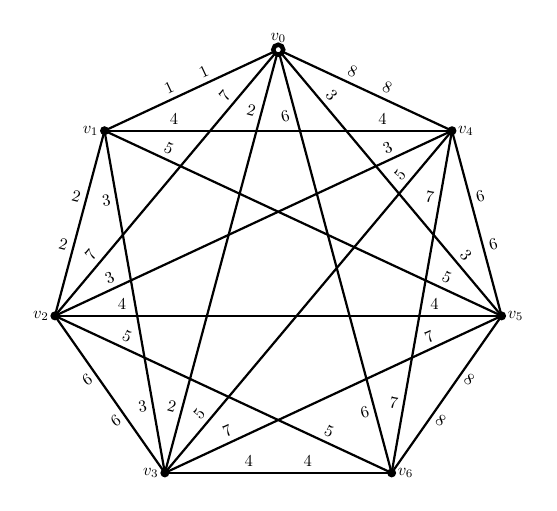
\begin{tikzpicture}[style=thick,scale=0.6, every node/.style={scale=0.6}]
    \coordinate (V3) at (-120:4.8cm);
    \coordinate (V2) at (-170:4.8cm);
    \coordinate (V1) at (140:4.8cm);
    \coordinate (V0) at (90:4.8cm);
    \coordinate (V4) at (40:4.8cm);
    \coordinate (V5) at (-10:4.8cm);
    \coordinate (V6) at (-60:4.8cm);
    
    \draw (V0) -- node [sloped,above,pos=0.4] {$1$} node [sloped,above,pos=0.6] {$1$} (V1);
    \draw (V0) -- node [sloped,above,pos=0.2] {$7$} node [sloped,above,pos=0.8] {$7$} (V2);
    \draw (V0) -- node [sloped,left,rotate=-90,pos=0.15] {$2$} node [sloped,left,rotate=-90,pos=0.85] {$2$} (V3);
    \draw (V0) -- node [sloped,above,pos=0.4] {$8$} node [sloped,above,pos=0.6] {$8$} (V4);
    \draw (V0) -- node [sloped,above,pos=0.2] {$3$} node [sloped,above,pos=0.8] {$3$} (V5);
    \draw (V0) -- node [sloped,left,rotate=90,pos=0.15] {$6$} node [sloped,left,rotate=90,pos=0.85] {$6$} (V6);
    
    \draw (V1) -- node [sloped,left,rotate=-90,pos=0.37] {$2$} node [sloped,left,rotate=-90,pos=0.63] {$2$} (V2);
    \draw (V1) -- node [sloped,left,rotate=90,pos=0.2] {$3$} node [sloped,left,rotate=90,pos=0.8] {$3$} (V3);
    \draw (V1) -- node [sloped,above,pos=0.2] {$4$} node [sloped,above,pos=0.8] {$4$} (V4);
    \draw (V1) -- node [sloped,above,pos=0.15] {$5$} node [sloped,above,pos=0.85] {$5$} (V5);
    % \draw (V1) -- node [sloped,left,rotate=-90] {$0$} (V6);
    
    \draw (V2) -- node [sloped,left,rotate=90,pos=0.37] {$6$} node [sloped,left,rotate=90,pos=0.63] {$6$} (V3);
    \draw (V2) -- node [sloped,above,pos=0.15] {$3$} node [sloped,above,pos=0.85] {$3$} (V4);
    \draw (V2) -- node [sloped,above,pos=0.15] {$4$} node [sloped,above,pos=0.85] {$4$} (V5);
    \draw (V2) -- node [sloped,above,pos=0.2] {$5$} node [sloped,above,pos=0.8] {$5$} (V6);
    
    \draw (V3) -- node [sloped,above,pos=0.15] {$5$} node [sloped,above,pos=0.85] {$5$} (V4);
    \draw (V3) -- node [sloped,above,pos=0.2] {$7$} node [sloped,above,pos=0.8] {$7$} (V5);
    \draw (V3) -- node [sloped,above,pos=0.37] {$4$} node [sloped,above,pos=0.63] {$4$} (V6);
    
    \draw (V4) -- node [sloped,right,rotate=90,pos=0.37] {$6$} node [sloped,right,rotate=90,pos=0.63] {$6$} (V5);
    \draw (V4) -- node [sloped,left,rotate=-90,pos=0.2] {$7$} node [sloped,left,rotate=-90,pos=0.8] {$7$} (V6);
    
    \draw (V5) -- node [sloped,right,rotate=-90,pos=0.37] {$8$} node [sloped,right,rotate=-90,pos=0.63] {$8$} (V6);
    
    \draw[fill=white,style=ultra thick] (V0) circle (3pt) node [above] {$v_0$};
    \draw[fill=black] (V1) circle (2pt) node [left] {$v_1$};
    \draw[fill=black] (V2) circle (2pt) node [left] {$v_2$};
    \draw[fill=black] (V3) circle (2pt) node [left] {$v_3$};
    \draw[fill=black] (V4) circle (2pt) node [right] {$v_4$};
    \draw[fill=black] (V5) circle (2pt) node [right] {$v_5$};
    \draw[fill=black] (V6) circle (2pt) node [right] {$v_6$};
  \end{tikzpicture}
  \end{center}
  \label{K7-minus-edge}
\end{figure}
$K_7-e$ գրաֆի $\beta$ ճիշտ կողային ներկումը $8$ գույներով, որտեղ $def( v_0,\beta)=def(K_7-e)=2$:
\end{frame}

\begin{frame}{$def(K_{1,m,n})$}
\begin{itemize}
\item (Ֆենգ, Հուանգ, 2007) $def\left(K_{1,1,n}\right)=0$, երբ $n$-ը զույգ է և $def\left(K_{1,1,n}\right)=1$, երբ $n$-ը կենտ է: 
\end{itemize}
\begin{theorem}[3.2.5]
Կամայական $m,n\in \mathbb{N}$ թվերի համար
\begin{center}
$def\left(K_{1,m,n}\right)=\left\{
\begin{tabular}{ll}
$0$, & երբ $(m+1,n+1)=1$,\\
$1$, & հակառակ դեպքում:\\
\end{tabular}%
\right.$
\end{center}
\end{theorem}
\end{frame}